\documentclass[11pt,a4paper]{article}

\usepackage[margin=2.4cm]{geometry}
\usepackage{amsmath,amssymb}
\usepackage{booktabs}
\usepackage{graphicx}
\usepackage{xcolor}
\usepackage{enumitem}
\usepackage{caption}
\usepackage{array}
\usepackage{listings}
\usepackage[colorlinks=true,linkcolor=blue!60!black,citecolor=blue!60!black,urlcolor=blue!60!black]{hyperref}

\graphicspath{{swing_height/fig/}}
\captionsetup{font=small,labelfont=bf,skip=4pt}
\setlist{itemsep=2pt,topsep=3pt}
\setlength{\emergencystretch}{3em}
\lstset{basicstyle=\ttfamily\small,columns=fullflexible,keepspaces=true,
        frame=single,framerule=0.3pt,rulecolor=\color{black!30},
        commentstyle=\color{black!55},xleftmargin=0.5em,xrightmargin=0.5em}

%% GENERATED by doc/swing_height/study.py
\newcommand{\ApexOff}{15.0}
\newcommand{\ApexOn}{23.4}
\newcommand{\LagOff}{55}
\newcommand{\LagOn}{33}
\newcommand{\RmsOff}{9.9}
\newcommand{\RmsOn}{3.4}
\newcommand{\HtdOff}{13.0}
\newcommand{\HtdOn}{\ensuremath{-1.9}}
\newcommand{\SapexOff}{0.83}
\newcommand{\SapexOn}{0.52}
\newcommand{\VtdOff}{\ensuremath{-0.10}}
\newcommand{\VtdOn}{\ensuremath{-0.11}}
\newcommand{\XOff}{4.2}
\newcommand{\XOn}{5.0}
\newcommand{\TauOff}{0.95}
\newcommand{\TauOn}{3.31}
\newcommand{\FfOn}{3.07}
\newcommand{\ClipOn}{0.21}
\newcommand{\PdOff}{1.00}
\newcommand{\PdOn}{0.87}
\newcommand{\ApexOnIdeal}{21.7}
\newcommand{\RmsOnIdeal}{1.6}
\newcommand{\ApexOffIdeal}{14.1}
\newcommand{\HtdOnIdeal}{0.7}
\newcommand{\ApexArmOff}{18.0}
\newcommand{\ApexArmOn}{34.0}
\newcommand{\ApexArmMatch}{24.5}
\newcommand{\HtdArmOn}{\ensuremath{-8.8}}
\newcommand{\RmsArmMatch}{3.6}
\newcommand{\HtdArmMatch}{\ensuremath{-3.4}}
\newcommand{\RmsArmOn}{12.1}
\newcommand{\HtdArmOff}{11.6}
\newcommand{\UnderOn}{\ensuremath{-2.3}}
\newcommand{\UnderArmOn}{\ensuremath{-8.8}}
\newcommand{\MMj}{\begin{bmatrix}0.0118 & 0.0001 & 0.0000\\0.0001 & 0.0131 & 0.0004\\0.0000 & 0.0004 & 0.0087\end{bmatrix}}
\newcommand{\MLaw}{\begin{bmatrix}0.0126 & 0.0001 & 0.0000\\0.0001 & 0.0140 & 0.0007\\0.0000 & 0.0007 & 0.0089\end{bmatrix}}
\newcommand{\MZero}{\begin{bmatrix}0.0115 & -0.0001 & -0.0000\\-0.0001 & 0.0139 & 0.0006\\-0.0000 & 0.0006 & 0.0089\end{bmatrix}}
\newcommand{\GMj}{\ensuremath{-0.021, -0.232, 0.006}}
\newcommand{\GLaw}{\ensuremath{-0.020, -0.257, 0.012}}
\newcommand{\LamZ}{5.72}
\newcommand{\LamX}{0.30}
\newcommand{\LamY}{0.37}
\newcommand{\LamZLinks}{0.58}
\newcommand{\SharePitch}{65}
\newcommand{\ShareKnee}{97}
\newcommand{\ShareAbd}{72}
\newcommand{\FfEquiv}{\ensuremath{4\times10^{-14}}}
\newcommand{\UnderArmOnAbs}{8.8}
\newcommand{\HtdArmOnAbs}{8.8}
\newcommand{\LinHtdArmOnAbs}{7.2}
\newcommand{\XArmOn}{17}
\newcommand{\LamZFive}{3.60}
\newcommand{\Wn}{8.4}
\newcommand{\WnHz}{1.33}
\newcommand{\Zeta}{0.42}
\newcommand{\LinApexOff}{11.2}
\newcommand{\LinHtdOff}{10.9}
\newcommand{\LinLagOff}{68}
\newcommand{\LinSapexOff}{0.87}
\newcommand{\LinApexOn}{20.0}
\newcommand{\LinHtdOn}{0.0}
\newcommand{\LinApexArmOff}{14.2}
\newcommand{\LinApexArmOn}{27.5}
\newcommand{\LinHtdArmOn}{\ensuremath{-7.2}}
\newcommand{\RobApex}{19.3}
\newcommand{\RobLag}{50}
\newcommand{\RobRms}{11.9}
\newcommand{\RobHtd}{12.7}
\newcommand{\RobN}{81}
\newcommand{\RobRefPk}{20.8}
\newcommand{\RobZlo}{1.8}
\newcommand{\RobApexAbs}{21.2}
\newcommand{\RobHtdAbs}{14.9}


\newcommand{\Jmat}{\mathbf{J}}
\newcommand{\Jbar}{\bar{\mathbf{J}}}
\newcommand{\Mmat}{\mathbf{M}}
\newcommand{\Kp}{\mathbf{K}_p}
\newcommand{\Kd}{\mathbf{K}_d}
\newcommand{\vp}{\mathbf{p}}
\newcommand{\vv}{\mathbf{v}}
\newcommand{\va}{\mathbf{a}}
\newcommand{\vq}{\mathbf{q}}
\newcommand{\vg}{\mathbf{g}}
\newcommand{\vc}{\mathbf{c}}
\newcommand{\vtau}{\boldsymbol{\tau}}
\newcommand{\ez}{\mathbf{e}_z}
\newcommand{\Nm}{\,N\,m}
\newcommand{\Nms}{\,N\,m/s}
\newcommand{\code}[1]{\texttt{#1}}

\title{\textbf{DOG6 Swing Height}\\[0.3em]
\large The Inertial Feedforward Off and On at a 20\,mm Apex:\\
one leg in MuJoCo, driven by the robot's own swing code}
\author{Eshou}
\date{26 October 2026}

\begin{document}
\maketitle

% ===========================================================================
\section*{Summary}

\begin{enumerate}[leftmargin=1.5em]
\item \textbf{The question.} The gait study (branch \code{gait-study-data})
flew the walk's swing with the inertial feedforward \emph{off}. On the robot the
swing foot reached about 20\,mm, but lifted about 50\,ms after the clock and was
still about 13\,mm in the air when the clock handed it the load. This note asks
what turning the feedforward (\code{--swing-ff}) on does at the same 20\,mm
apex, with everything else as flown.

\item \textbf{The setup.} The robot's right-rear (RR) leg is hung up in MuJoCo.
Its masses are the weighed ones and its frame is the robot's
(\S\ref{sec:model}). The leg is driven by the hardware swing bench's own code
(\code{hw.swing\_bench.SwingBench}, the gait clock and the torque gate), passed
through an emulated CAN round robin, encoder, velocity filter and current loop
(\S\ref{sec:hw2sim}). The settings are the study's: a 160\,ms swing, a 20\,mm
apex, gains 150/150/400\,N/m and 6/6/40\,N\,s/m, a 300\Nms{} slew and the
FOLD2 stance at 160\,mm. For this arc the bench's swing torque is the walk's
to $\FfEquiv$\Nm.

\item \textbf{Feedforward off: the foot is late and short.} The PD has to make
the force out of tracking error. On a foot that weighs \LamZ\,kg in $z$ (the
reflected rotor, \S\ref{sec:mass}) the PD is a \WnHz\,Hz spring, far too slow
for a 160\,ms arc. The apex is \ApexOff\,mm at $s=\SapexOff$, the foot
crosses 4\,mm after \LagOff\,ms, and it is still \HtdOff\,mm up when the clock
lands it.

\item \textbf{Feedforward on: the foot follows the arc and lands on time.} The
apex is \ApexOn\,mm at $s=\SapexOn$, the tracking error falls from \RmsOff{} to
\RmsOn\,mm rms, and the height at the clock's touchdown is \HtdOn\,mm instead
of \HtdOff. The 3.4\,mm of overshoot comes from the hardware chain: with an
ideal chain the apex is \ApexOnIdeal\,mm and the rms error \RmsOnIdeal\,mm.

\item \textbf{The simulation reproduces the robot with feedforward off.} Against
\RobN{} RR swings from the study's logs, the lag (\RobLag{} vs \LagOff\,ms) and
the height at touchdown (\RobHtd{} vs \HtdOff\,mm) agree. The robot's apex is
4\,mm higher (\RobApex{} vs \ApexOff\,mm), a gap the leg model does not
account for (\S\ref{sec:robot}).

\item \textbf{The armature is the feedforward's gain, and here it is right.}
The rotor term, 0.0085\,kg\,m$^2$, is the MG5010-i10 datasheet's rotor inertia
times the 10:1 ratio squared. DOG5 and DOG6 use the same motor. $\Mmat_0$ is
built on the same number, so model and plant agree on the term that dominates
$\Mmat$. As a sensitivity, if the leg's effective inertia were lower than the
datasheet's (a rotor term of 0.005, as one 2026-09-25 bench reading would
imply), $\Mmat_0$ would overdrive the leg: the apex reaches \ApexArmOn\,mm and
the foot comes down \UnderArmOnAbs\,mm below its site (\S\ref{sec:sens}).

\item \textbf{Recommendation.} Turn the feedforward on for the 20\,mm, 160\,ms
swing. The default $\Mmat_0$ already uses the datasheet rotor. Before walking,
run one hung-up bench check with the feedforward on and compare it with this
note's prediction (apex about 23\,mm, $h_{td}$ about $-2$\,mm). The feedforward
removes the late landing the gait study traced its tips to.
\end{enumerate}

% ===========================================================================
\section{Scope and notation}

This note covers one swing leg with the trunk pinned, which is the robot hung up
on the bench. No floor, no stance law and no trunk motion are modelled. The
contact a real landing makes is therefore not here. What is here is whether the
foot follows the arc, and where it is when the clock says it is down.

\begin{tabbing}
\hspace{3.2cm}\=\kill
$\vq = (q_a, q_p, q_k)$ \> RR joints: abduction, hip pitch, knee \\
$\vp = \mathrm{FK}(\vq)$ \> foot-ball centre, trunk frame ($x$ forward, $y$ left, $z$ up) \\
$\Jmat$, $\Jbar$ \> foot Jacobian ($3\times3$); its pitch and knee columns ($3\times2$) \\
$\Jbar^+$ \> $(\Jbar^\top\Jbar)^{-1}\Jbar^\top$ \\
$\Mmat(\vq)$, $\Mmat_0$ \> joint-space inertia; the constant the feedforward multiplies by \\
$\vc(\vq,\dot\vq)$, $\vg(\vq)$ \> Coriolis/centrifugal and gravity torques \\
$\Lambda$ \> foot apparent mass, $(\Jmat\Mmat^{-1}\Jmat^\top)^{-1}$ \\
$T_g$, $d$, $T$ \> gait period 0.8\,s, duty 0.8, swing $T = (1-d)T_g = 160$\,ms \\
$s = (t - t_{lo})/T$ \> swing progress: 0 at the clock's liftoff, 1 at its touchdown \\
$H$ \> commanded swing height (apex), 20\,mm
\end{tabbing}

\paragraph{What ``swing height'' means here, and how it is measured.} $H$ is the
apex of the reference arc above the foot's resting site, in the trunk frame
(\S\ref{sec:arc}). The height the foot \emph{reaches} is read from forward
kinematics of the encoders, exactly as the robot's log reads it. Four numbers
per swing use the gait study's definitions (\code{doc/gait\_study/analyse.py}),
with the swing window being the clock's, from liftoff to touchdown:
\begin{itemize}[leftmargin=1.5em]
\item \textbf{apex}: the largest height in the window, and $s_{apex}$, where it occurs;
\item \textbf{lag}: from the clock's liftoff until the foot is 4\,mm up;
\item \textbf{rms}: $|\vp_{ref} - \vp|$ over the window, in 3-D;
\item $\boldsymbol{h_{td}}$: the height on the sweep the clock lands the foot.
This is the foot's position when the allocator starts loading it.
\end{itemize}
On the bench, heights are measured from the resting site. That is the arc's own
zero, because there is no floor. The first two swings of each 40-swing run are
dropped, and the rest are summarised as medians.

% ===========================================================================
\section{The model}
\label{sec:model}

\subsection{The leg}

The plant is \code{doc/swing\_height/model/leg\_RR.xml}, generated by
\code{build\_leg.py}. It is DOG6's RR leg alone, with the hip body attached to
the world (the trunk pinned) and gravity on.

\begin{table}[h]
\centering\small
\begin{tabular}{llrrrl}
\toprule
body & carries & CAD & weighed & scale & CoM, body frame, mm \\
\midrule
\code{hip\_RR} & adapter + pitch motor & 0.400\,kg & 0.385\,kg & 0.963 & $(-25.7,\ 0.0,\ -2.3)$ \\
\code{thigh\_RR} & link + knee motor & 0.412\,kg & 0.391\,kg & 0.949 & $(-90.0,\ 0.0,\ 8.4)$ \\
\code{shin\_RR} & shin + foot & 0.072\,kg & 0.040\,kg & 0.558 & $(-64.0,\ 0,\ -7.2)$ \\
\bottomrule
\end{tabular}
\caption{The leg. Body offsets, hinge axes, CoMs and the shape of each inertia
tensor come from \code{sim/model/dog6.xml}. The masses are weighed (adapter
55\,g and link 61\,g, plus a 330\,g motor each; shin with foot 40\,g), and each
CAD tensor is scaled by weighed\,/\,CAD mass. This is the recipe of
\code{leg\_swing/leg.xml}. Every hinge carries an armature of
0.0085\,kg\,m$^2$: the MG5010-i10 datasheet's rotor inertia,
$8.5\times10^{-5}$\,kg\,m$^2$, times $10^2$. DOG5 and DOG6 use the same motor.
There is no
damping, friction or contact, and three motors of gear 1 drive the hinges.
The abduction motor's stator is on the trunk, so its mass is not in the leg;
its rotor is in \code{hip\_abd\_RR}'s armature.}
\label{tab:leg}
\end{table}

\paragraph{Why not \code{leg.xml} itself.} \code{leg.xml} was cut from the
2026-09-07 extraction, \code{dog6\_description/}\allowbreak\code{dog6.xml}
under \code{D:/mujoco}. That was before
\code{sim/model/dog6.xml}'s hand fix of 2026-09-15, which rolled every leg
body's inertial and sites $180^\circ$ about $x$ because the flat zero had been
folded the wrong way: $(x,y,z)\to(x,-y,-z)$, and $I_{xy}$ and $I_{xz}$ negated.
In \code{leg.xml} every link CoM and the foot site therefore have the opposite
$z$. At the same joint angles its foot is up to 10\,mm from where the robot's
kinematics put it, and its abduction gravity torque has the opposite sign. The
masses are right but the frame is not the robot's, so \code{leg\_RR.xml} keeps
the first and replaces the second.

\paragraph{The gate.} \code{build\_leg.py} checks the model against the
controller's own chain over 2000 random joint vectors on the full circle. On a
CAD-mass copy, the foot site matches \code{hw.kinematics.foot\_position} to
$1\times10^{-16}$\,m, the site Jacobian matches \code{foot\_jacobian} to
$1\times10^{-16}$, and MuJoCo's gravity torque matches the law's closed form to
$3\times10^{-16}$\Nm. With the weighed masses the gravity torques differ by up
to 0.07\Nm. That is the real model error the law carries, and it is kept.

\subsection{The pose}

The study flew FOLD2 at 160\,mm (trunk bottom above the floor). At that hold
the RR joints are $\vq_{hold} = (90^\circ,\ 51.74^\circ,\ 53.12^\circ)$ and the
foot is at $(-219.5,\ -65.0,\ -180.0)$\,mm in the trunk frame. With
abduction at $90^\circ$, the pitch and knee axes lie along trunk $y$, so the
leg moves in the trunk $x$--$z$ plane (Figure~\ref{fig:model}):
\[
\Jmat(\vq_{hold}) = \begin{bmatrix}
0 & 0.1800 & 0.1015\\ 0.1800 & 0 & 0\\ -0.0050 & -0.0350 & 0.0269
\end{bmatrix}\ \text{m/rad}.
\]
The bottom row is the problem this note is about. A vertical foot motion comes
almost entirely from the knee and pitch, through levers of only 27 and 35\,mm
per radian.

\begin{figure}[h]
\centering
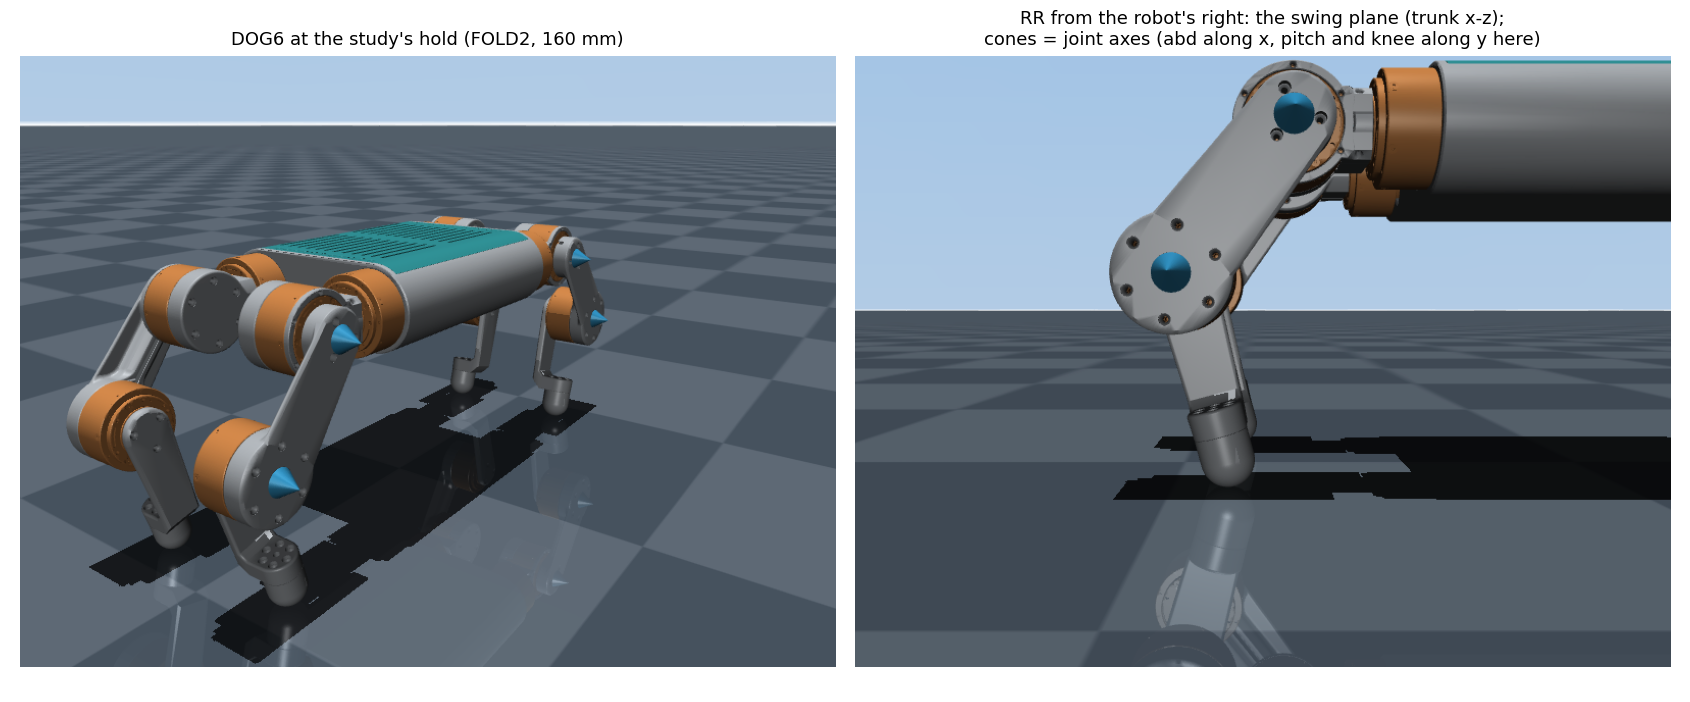
\includegraphics[width=\linewidth]{model.png}
\caption{DOG6 at the study's hold (left). On the right is the RR leg seen from
the robot's right side, the plane it swings in. The cones mark the joint axes.
In the simulation only this leg exists, and its hip is pinned where the trunk
would be.}
\label{fig:model}
\end{figure}

% ===========================================================================
\section{The mass matrix and gravity, from MuJoCo}
\label{sec:mass}

\subsection{What MuJoCo computes}

The leg obeys
\begin{equation}
\Mmat(\vq)\,\ddot\vq + \vc(\vq,\dot\vq) + \vg(\vq) = \vtau ,
\qquad \Mmat(\vq) = \Mmat_{links}(\vq) + I_a\,\mathbf{1},
\label{eq:eom}
\end{equation}
with $I_a = 0.0085$\,kg\,m$^2$, the rotor reflected through the 10:1 gearbox
(datasheet rotor inertia $8.5\times10^{-5}$\,kg\,m$^2$ times $10^2$). It is
constant, so it adds to the diagonal of $\Mmat$ and contributes nothing to
$\vc$ or $\vg$. One call to \code{mj\_forward} computes $\Mmat$ by the composite
rigid-body algorithm, stored sparse in \code{d.qM}. It computes the bias
$\vc+\vg$ by recursive Newton--Euler, stored in \code{d.qfrc\_bias}. At
$\dot\vq = 0$ the bias is gravity alone. For a given $\ddot\vq$,
\code{mj\_inverse} returns the whole left side of \eqref{eq:eom}:

\begin{lstlisting}[language=Python]
m = mujoco.MjModel.from_xml_path("doc/swing_height/model/leg_RR.xml")
d = mujoco.MjData(m)
d.qpos[:] = q; d.qvel[:] = 0.0
mujoco.mj_forward(m, d)           # FK; CRBA -> d.qM; RNE -> d.qfrc_bias
M = np.zeros((3, 3))
mujoco.mj_fullM(m, M, d.qM)       # dense M(q), armature on the diagonal
g = d.qfrc_bias.copy()            # c(q, 0) + g(q) = g(q), the holding torque
d.qvel[:] = qd; d.qacc[:] = qdd   # a point on the arc
mujoco.mj_inverse(m, d)           # qfrc_inverse = M qdd + c(q, qd) + g(q)
\end{lstlisting}

The controller does not run MuJoCo. Its gravity term is a closed form over the
CAD masses (\code{hw.balance.torque.leg\_gravity\_torque}), and its $\Mmat_0$ is
\code{sim.leg\_dynamics.mass\_matrix}, an RNEA over the CAD inertials, evaluated
once at the front-left leg's lift pose with the armature added. The repository's
self-tests gate both against MuJoCo on the CAD model, and the gate above
repeats that for this leg.

\subsection{The numbers at the hold}

\begin{gather*}
\Mmat_{\text{MuJoCo}}(\vq_{hold}) = \MMj, \qquad
\Mmat_{\text{law}}(\vq_{hold}) = \MLaw, \\[4pt]
\Mmat_0 = \MZero \qquad (\text{kg\,m}^2).
\end{gather*} The first is the weighed leg in MuJoCo, the second the law's RNEA
on CAD masses at the same pose, and the third the constant the feedforward
uses. The armature is \ShareAbd, \SharePitch{} and \ShareKnee\,\% of the
abduction, pitch and knee diagonals. The off-diagonal terms are below
0.0004. So the constant $\Mmat_0$ is within 6\,\% of the true $\Mmat$ on the
pitch and 2\,\% on the knee, and its error is mostly the CAD-versus-weighed
link masses. The rotor dominates that error. Gravity is
$\vg = (\GMj)$\Nm{} in MuJoCo against $(\GLaw)$\Nm{} in the law.

\paragraph{The apparent mass at the foot.} Mapped through $\Jmat$, the joint
inertia becomes $\Lambda = (\Jmat\Mmat^{-1}\Jmat^\top)^{-1}$, whose diagonal is
(\LamX, \LamY, \LamZ)\,kg in $x$, $y$ and $z$. Without the armature it would be
\LamZLinks\,kg in $z$. The rotor, seen through the knee's 27\,mm/rad lever,
makes the foot ten times heavier vertically than the leg actually is. Every
result below follows from this.

\subsection{What the arc asks for}

Figure~\ref{fig:dyn} runs MuJoCo's inverse dynamics along the 20\,mm, 160\,ms
arc. $\Mmat\ddot\vq$ peaks at 2.55\Nm{} on the pitch and 3.08\Nm{} on the knee.
Gravity is at most 0.29\Nm, and $\vc(\vq,\dot\vq)$ is 0.006\Nm, which is why the
law leaves it out. The law's feedforward plus its gravity overlays MuJoCo's
answer, and its torque \emph{rate} peaks at 357 and 424\Nms{} against the
gate's 300.

\begin{figure}[h]
\centering
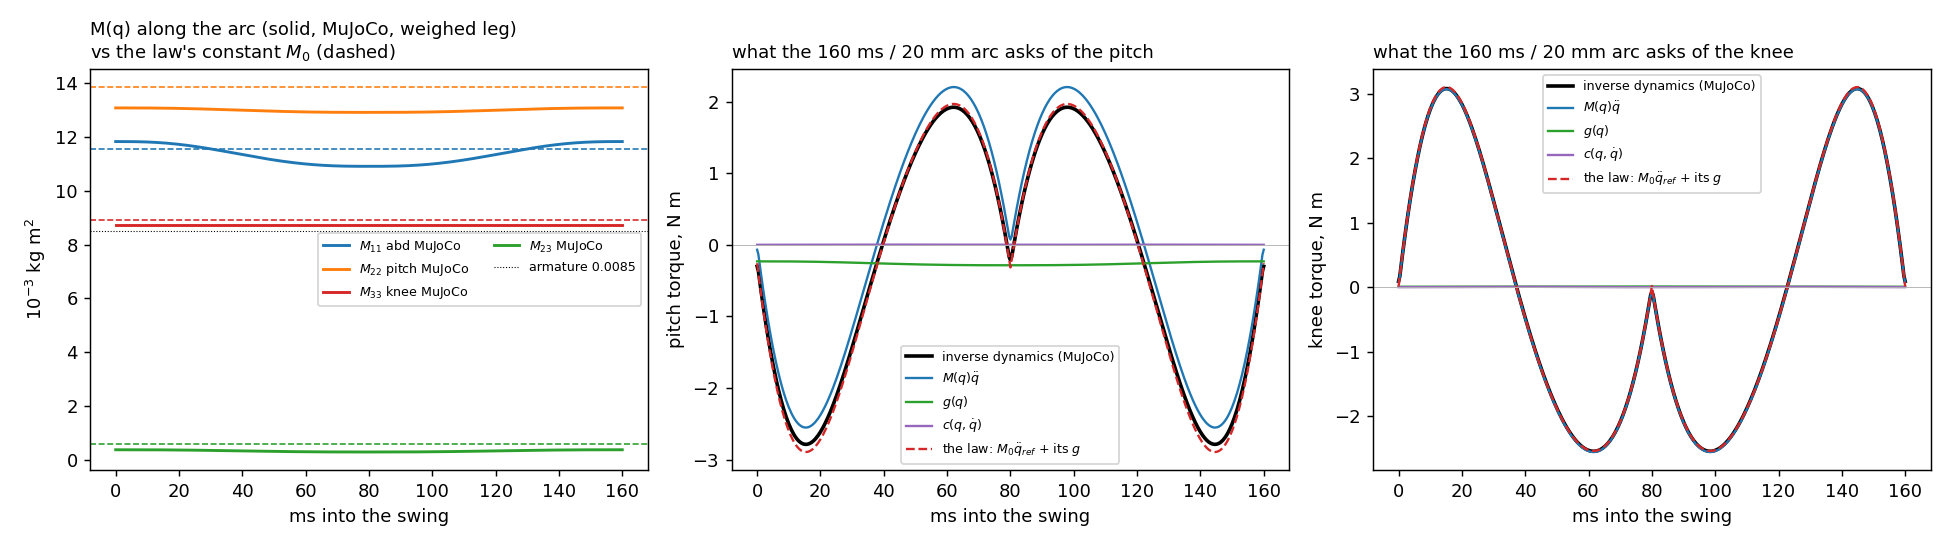
\includegraphics[width=\linewidth]{arc_dynamics.png}
\caption{Left: $\Mmat(\vq)$ along the arc from MuJoCo (solid) against the
law's constant $\Mmat_0$ (dashed). Middle and right: MuJoCo's inverse dynamics
split into $\Mmat\ddot\vq$, $\vg$ and $\vc$, and the law's
$\Mmat_0\ddot\vq_{ref}$ plus its own gravity (red dashed). The notch at the
apex is the arc's: both quintic halves end with zero acceleration.}
\label{fig:dyn}
\end{figure}

% ===========================================================================
\section{The swing reference: the commanded height}
\label{sec:arc}

The gait clock (\code{hw.balance.gait.TrotGait}: period 0.8\,s, duty 0.8,
contact ramp 0.15, FL+RR on one diagonal) lifts RR for $T = 160$\,ms every
cycle. In that window the foot follows an arc in the trunk frame that starts and
ends on the resting site $\vp_0$, the hold's foot position, and rises straight
up (\code{sim.cmpc.swing.SwingTrajectory}):
\begin{equation}
\vp_{ref}(s) = \vp_0 + z(s)\,\ez,\qquad
z(s) = \begin{cases} H\,\sigma(2s) & s < \tfrac12\\ H\,\sigma(2-2s) & s \ge \tfrac12\end{cases},
\qquad \sigma(u) = 10u^3 - 15u^4 + 6u^5 .
\label{eq:arc}
\end{equation}
Each half has zero velocity and zero acceleration at both ends. The foot leaves
and arrives at rest, and $\va_{ref}$ has no step that the feedforward would turn
into a torque step. At $H = 20$\,mm and $T = 160$\,ms the arc peaks at
$|\dot z| = 3.75H/T = 0.47$\,m/s at $s = 0.25$ and $0.75$, and at
$|\ddot z| = 23.1H/T^2 = 18.0$\,m/s$^2$.

% ===========================================================================
\section{The swing control law}
\label{sec:law}

While the clock has the leg in swing, the bench (\code{hw.swing\_bench}) sends
\begin{equation}
\vtau = \vg_{law}(\vq)
\;+\; \Jmat^\top\!\big[\Kp(\vp_{ref} - \vp) + \Kd(\vv_{ref} - \Jmat\dot\vq)\big]
\;+\; \underbrace{\Mmat_0\,\ddot\vq_{ref}}_{\text{\code{--swing-ff}}},
\label{eq:law}
\end{equation}
with $\Kp = \mathrm{diag}(150,150,400)$\,N/m and $\Kd = \mathrm{diag}(6,6,40)$\,N\,s/m
(\code{config.KP/KD\_SWING\_WALK}). $\vp$ and $\Jmat$ come from this sweep's
encoders through \code{balance.state.read}, and $\dot\vq$ from the runner's
40\,Hz low-pass of the encoder difference. In stance the same impedance holds
the foot at $\vp_0$ with $\vv_{ref}=0$. The request then passes the safety
gate: a 9\Nm{} clip and a 300\Nms{} slew on every joint.

\paragraph{What the PD alone can do.} Along $z$, \eqref{eq:law} without the
feedforward is a spring and damper on the foot's apparent mass:
\[
\omega_n = \sqrt{K_{p,z}/\Lambda_{zz}} = \Wn\ \text{rad/s}\ (\WnHz\ \text{Hz}),\qquad
\zeta = \frac{K_{d,z}}{2\sqrt{K_{p,z}\Lambda_{zz}}} = \Zeta .
\]
Its natural period is 750\,ms, against a 160\,ms arc. In force terms, the arc
needs $\Lambda_{zz}\ddot z \approx 100$\,N at the foot at its peaks. The PD's
velocity term $K_{d,z}\dot z_{ref}$ gives at most 19\,N, and the rest has to
come from a position error that takes most of the swing to build.

% ===========================================================================
\section{The feedforward}
\label{sec:ff}

\code{--swing-ff} adds the torque the arc needs, open loop
(\code{hw.balance.swing.swing\_feedforward}):
\begin{equation}
\dot\vq_{ref} = \Jbar^+\vv_{ref},\qquad
\ddot\vq_{ref} = \Jbar^+\big(\va_{ref} - \dot\Jmat\dot\vq_{ref}\big),\qquad
\vtau_{ff} = \Mmat_0\,\ddot\vq_{ref}.
\label{eq:ff}
\end{equation}
\begin{itemize}[leftmargin=1.5em]
\item The solve uses the pitch and knee columns of the \emph{measured}
Jacobian, and abduction gets nothing. The arc has no $y$ in it.
\item $\dot\Jmat\dot\vq_{ref}$ is one more Jacobian at
$\vq + \epsilon\dot\vq_{ref}$ ($\epsilon = 10^{-4}$\,s), differenced. Without it
the chain's curvature pulls the foot off the vertical line.
\item $\Mmat_0$ is the constant of \S\ref{sec:mass}. The term $\vc\,\dot\vq$ is
left out (0.006\Nm).
\item The walk's form (\code{swing\_control.inertial\_feedforward}) solves
through all three columns, $\ddot\vq_{ref} = \Jmat^{-1}(\va_{ref} -
\dot\Jmat\dot\vq_{ref})$. At this pose and on this arc it equals
\eqref{eq:ff} to $\FfEquiv$\Nm, and the PD is the same expression. So the
bench's swing \emph{is} the swing the gait study flew.
\end{itemize}
Along the arc $\vtau_{ff}$ peaks at 2.6\Nm{} on the pitch and 3.1\Nm{} on the
knee (Figure~\ref{fig:dyn}).

\paragraph{What sets the height the foot reaches.} Reduce the swing to its $z$
axis, a mass $\Lambda_{zz}$ on the PD with the feedforward's own idea of that
mass, $\Lambda_0$, multiplying $\ddot z_{ref}$:
\begin{equation}
\frac{Z(s)}{Z_{ref}(s)} = \frac{\Lambda_0 s^2 + K_{d,z}s + K_{p,z}}{\Lambda_{zz}s^2 + K_{d,z}s + K_{p,z}} .
\label{eq:tf}
\end{equation}
\begin{itemize}[leftmargin=1.5em]
\item \textbf{FF off} ($\Lambda_0 = 0$): a second-order low-pass with a zero.
The 160\,ms arc is above its corner, so it is cut down and delayed. This model
alone gives an apex of \LinApexOff\,mm at $s=\LinSapexOff$, $h_{td}$ =
\LinHtdOff\,mm and a lag of \LinLagOff\,ms.
\item \textbf{FF on, mass right} ($\Lambda_0 = \Lambda_{zz}$): the ratio is 1.
The foot follows the arc exactly (\LinApexOn\,mm, on time).
\item \textbf{FF on, mass wrong} ($\Lambda_0 = k\Lambda_{zz}$): the
high-frequency gain is $k$. If the leg's effective rotor term were 0.005
instead of the datasheet's 0.0085, $\Lambda_{zz}$ would fall to \LamZFive\,kg
while $\Lambda_0$ stays at \LamZ, so $k = 1.59$. The apex becomes \LinApexArmOn\,mm, and when the clock lands the
foot it is \LinHtdArmOnAbs\,mm below its site.
\end{itemize}
Without the feedforward, then, the swing height is a filter's output and has
little to do with $H$. With it, the height is $H$ times the ratio of the model's
mass to the leg's. The full simulation below adds what this model omits: the
delay, the slew, the coupling into $x$, and the bench's own ringing.

% ===========================================================================
\section{From the robot's code to the simulator}
\label{sec:hw2sim}

\code{doc/swing\_height/hwsim\_leg.py} is \code{hw.swing\_bench.run}'s loop
with MuJoCo in place of \code{can0}, following the pattern of
\code{doc/crouch\_trot/hwsim.py}. Table~\ref{tab:chain} lists what runs and
what is emulated.

\begin{table}[h]
\centering\small
\begin{tabular}{p{4.9cm}p{10.6cm}}
\toprule
\multicolumn{2}{l}{\textbf{runs unmodified, imported from the repository}}\\
\code{hw.swing\_bench.SwingBench} & phases limp $\to$ pose $\to$ hold $\to$ swing; the arc, the PD, \code{--swing-ff}, the per-swing report \\
\code{hw.balance.gait.TrotGait} & the clock: period 0.8\,s, duty 0.8, ramp 0.15, no settle \\
\code{hw.safety.SafetyGate} & 1\,s torque ramp, 9\Nm{} clip, 300\Nms{} slew, soft limits, \code{estop\_reason} \\
\code{hw.balance.state.read} & FK and Jacobian from the measured joints \\
\midrule
\multicolumn{2}{l}{\textbf{emulated} (numbers from \code{hwsim.py} unless stated)}\\
sweep & 5.51\,ms, 12 slots. This is the period the study's logs measured on the robot (5.43--5.54\,ms), not the nominal 4\,ms. The velocity filter keeps the code's constant, which is computed for 250\,Hz \\
CAN round robin & the law runs at slot 0 and takes 0.5\,ms. Motor $k$'s frame lands at $\max(k\cdot\text{slot}, 0.5\,\text{ms}) + 0.15$\,ms. RR is motors 9--11, so its torque lands 4.3--5.2\,ms after the law ran. Each reply is sampled at landing and read at the next slot 0. Every other sweep one motor (rotating) gets a status request instead of a command \\
encoder, current loop & 360/65535$^\circ$ per LSB; first-order lag 0.3\,ms; current quantised to 1/206.04\Nm{} and saturated at 9.94\Nm \\
position mode & the pose phase only: driver PD 120\Nm/rad and 3\Nm\,s/rad, reference slewed at the frame's speed cap \\
physics & MuJoCo, implicitfast, 0.46\,ms steps (12 per sweep) \\
\bottomrule
\end{tabular}
\caption{The hardware-in-the-loop chain. \code{Chain(ideal=True)} turns the
emulated part off: the law reads the true $\vq,\dot\vq$ and its torque reaches
the joint at once. Comparing against it isolates what the chain costs.}
\label{tab:chain}
\end{table}

One setting is applied from outside: the bench knows only the lift and fold
postures, so its held pose and resting sites are replaced with FOLD2 at 160\,mm,
using the same arithmetic \code{swing\_bench.bench\_pose} applies to the fold.
Each run is operated as on the robot: ENTER at once (pose), the hold's
1\,s ramp and 2\,s of hold, ENTER (swing), 40 swings, the bench's own stop at
the next four-foot window, and 1\,s of hold.

% ===========================================================================
\section{Results: feedforward off against on}
\label{sec:results}

\begin{table}[h]
\centering\small
\begin{tabular}{lrrrrrrrrr}
\toprule
 & apex & $s_{apex}$ & lag & rms & $h_{td}$ & $v_{z,td}$ & $|x|$ & $\hat\tau$ & clip \\
 & mm & & ms & mm & mm & m/s & mm & N\,m & N\,m \\
\midrule
\textbf{FF off} & 15.0 & 0.83 & 55 & 9.9 & 13.0 & $-$0.10 & 4.2 & 0.95 & 0.00 \\
\textbf{FF on} & 23.4 & 0.52 & 33 & 3.4 & $-$1.9 & $-$0.11 & 5.0 & 3.31 & 0.21 \\
\midrule
FF off, ideal chain & 14.1 & 0.79 & 55 & 9.2 & 12.2 & $-$0.08 & 3.3 & 0.87 & 0.00 \\
FF on, ideal chain & 21.7 & 0.48 & 28 & 1.6 & 0.7 & $-$0.01 & 1.0 & 3.11 & 0.00 \\
\bottomrule
\end{tabular}

\caption{Per swing, medians over swings 3--40. Heights are above the resting
site. $\hat\tau$ is the largest torque sent, and clip is the most the slew held
back. The upper block is the emulated hardware chain, the lower the ideal one.}
\label{tab:results}
\end{table}

\begin{figure}[p]
\centering
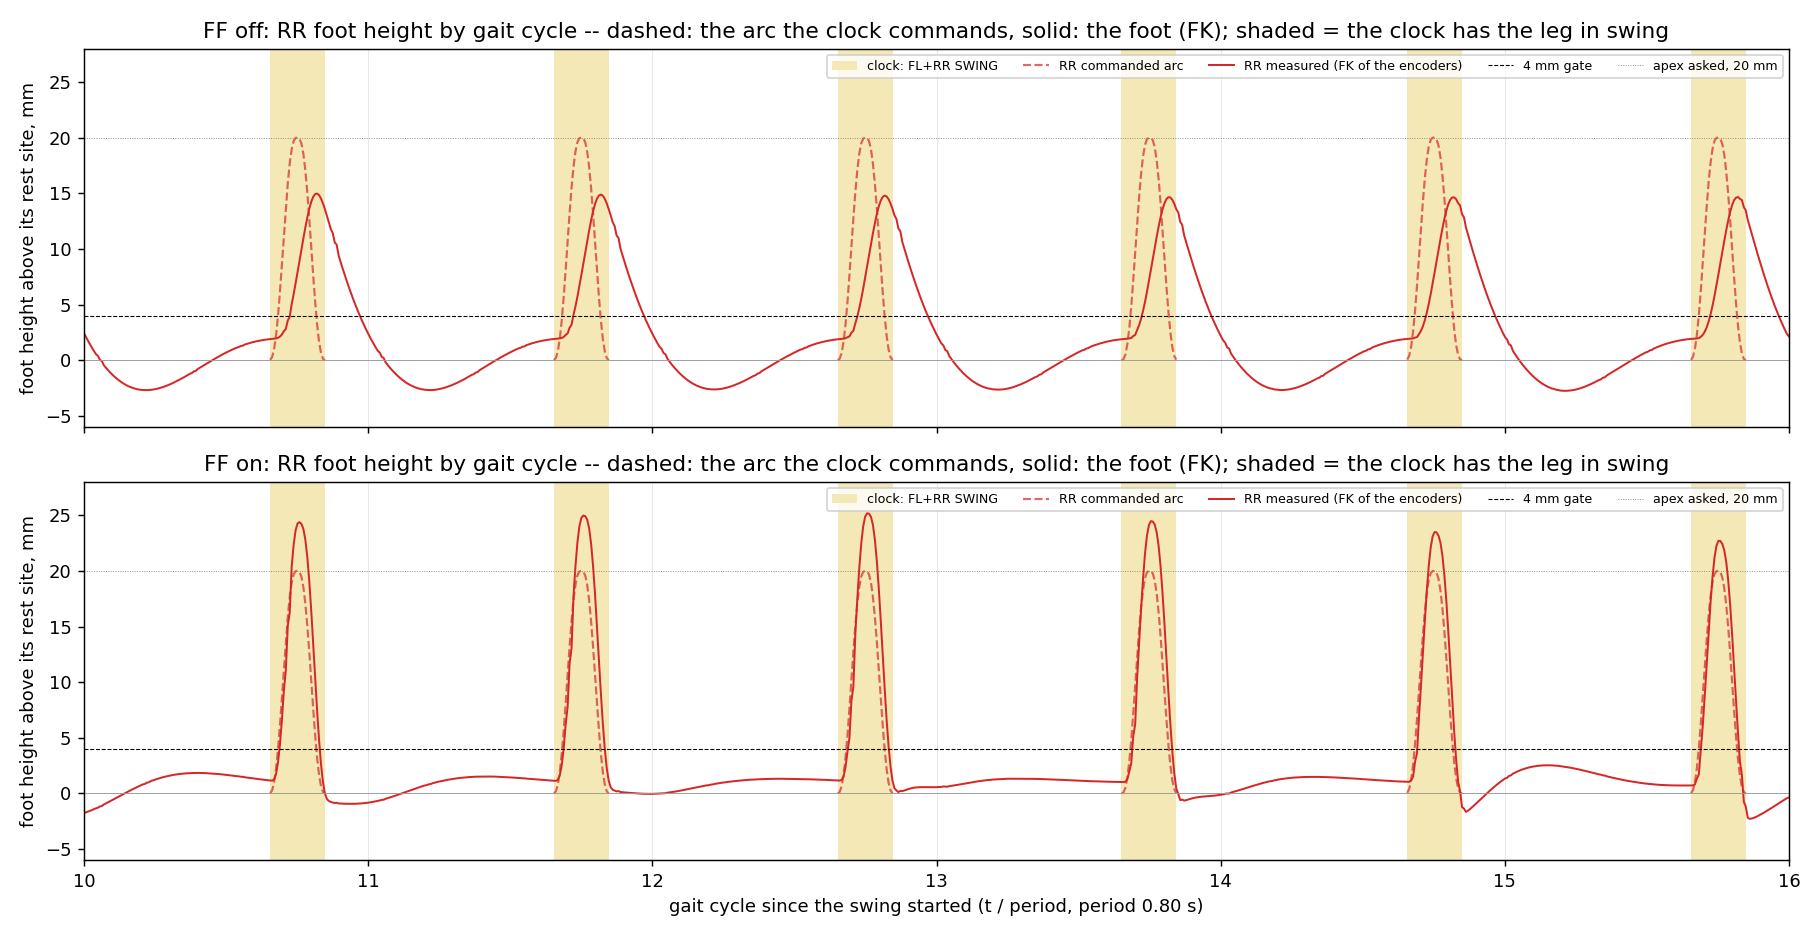
\includegraphics[width=\linewidth]{height_one_axis.png}
\caption{Six gait cycles, drawn as the gait study's figure 10. Dashed: the arc
the clock commands. Solid: the foot from the encoders. Shaded: the clock has
the leg in swing. Off, the foot rises only as the arc is ending and comes down
in the clock's stance. On, it follows the arc inside the window.}
\label{fig:oneaxis}
\vspace{1em}
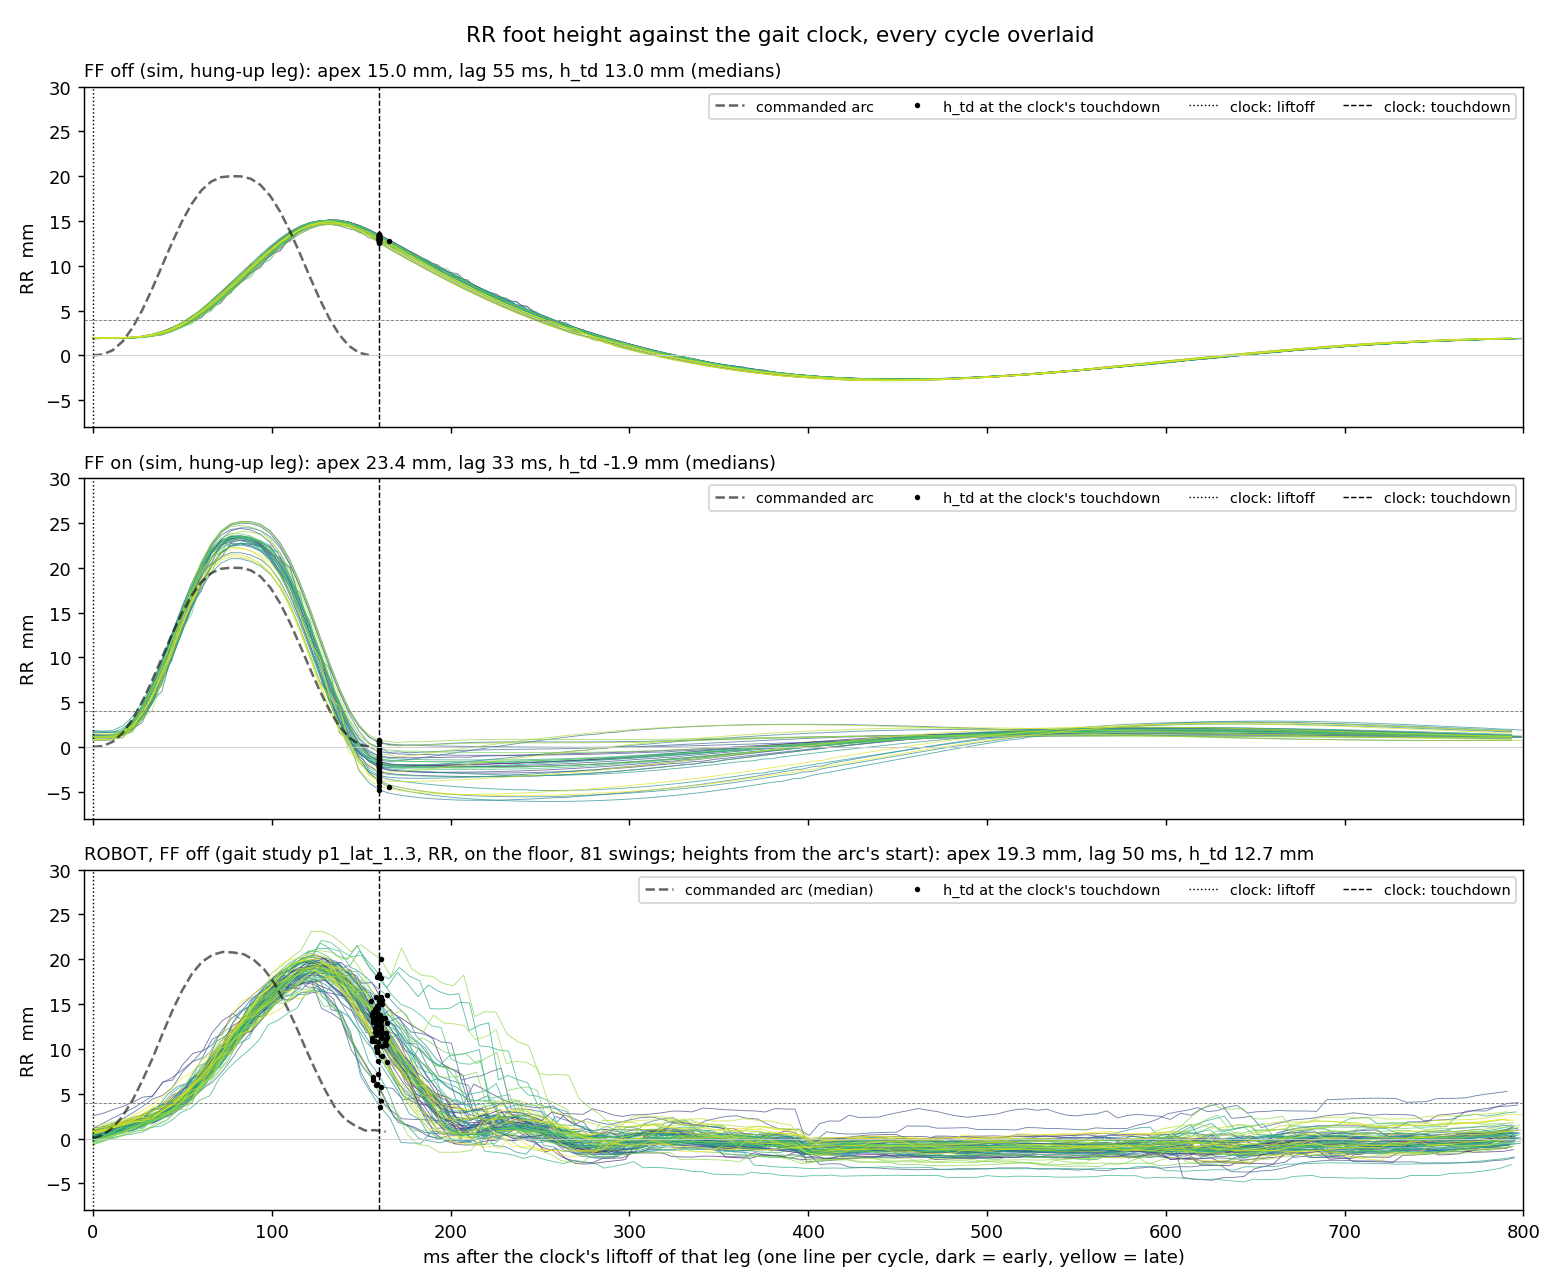
\includegraphics[width=\linewidth]{height_vs_phase.png}
\caption{Every cycle overlaid on the leg's own clock (the study's figure 8), with
the robot's FF-off swings below for comparison. Black dots: the height when the
clock lands the foot.}
\label{fig:phase}
\end{figure}

\paragraph{Feedforward off.} The foot does what \eqref{eq:tf} predicts for a
low-pass. It starts late (\LagOff\,ms to 4\,mm), peaks at \ApexOff\,mm only at
$s=\SapexOff$, and at the clock's touchdown it is still \HtdOff\,mm up and
descending (Figures~\ref{fig:oneaxis}, \ref{fig:phase}). It is back below
4\,mm only 94\,ms, and below 1\,mm 143\,ms, into what the clock already calls
stance. The torque stays small
(\TauOff\Nm{} peak; Figure~\ref{fig:torque}) because the PD never builds a large
error. The swing is not short of torque; the law simply never asks for it.

\paragraph{Feedforward on.} The torque arrives when the arc needs it. The
request is \FfOn\Nm{} of feedforward and \PdOn\Nm{} of PD at their peaks. The
foot crosses 4\,mm at \LagOn\,ms, peaks at $s=\SapexOn$, and is at \HtdOn\,mm
when the clock lands it, which is within a few millimetres of its site and on
time. The tracking error falls from \RmsOff{} to \RmsOn\,mm rms
(Figure~\ref{fig:err}).

\paragraph{The overshoot is the chain's.} With the ideal chain, the same law
gives \ApexOnIdeal\,mm and \RmsOnIdeal\,mm rms. Three things add the rest:
\begin{itemize}[leftmargin=1.5em]
\item \textbf{The delay.} The torque lands one sweep (about 5\,ms) after the
state it was computed from.
\item \textbf{The slew.} The arc's torque rate (up to 424\Nms) exceeds the 300
allowed, and the gate clips \ClipOn\Nm{} at the notch and the reversals.
\item \textbf{$\Mmat_0$ is slightly too large.} It is 6\,\% high on the pitch.
\end{itemize}
The swing-to-swing spread in Figure~\ref{fig:cycles} has a slow beat. The
status request skips one motor's command every 24 sweeps, and its phase against
the 145.2-sweep cycle drifts. With the status requests switched off, the
FF-on apex spread falls from 1.0 to 0.3\,mm (standard deviation).

\begin{figure}[p]
\centering
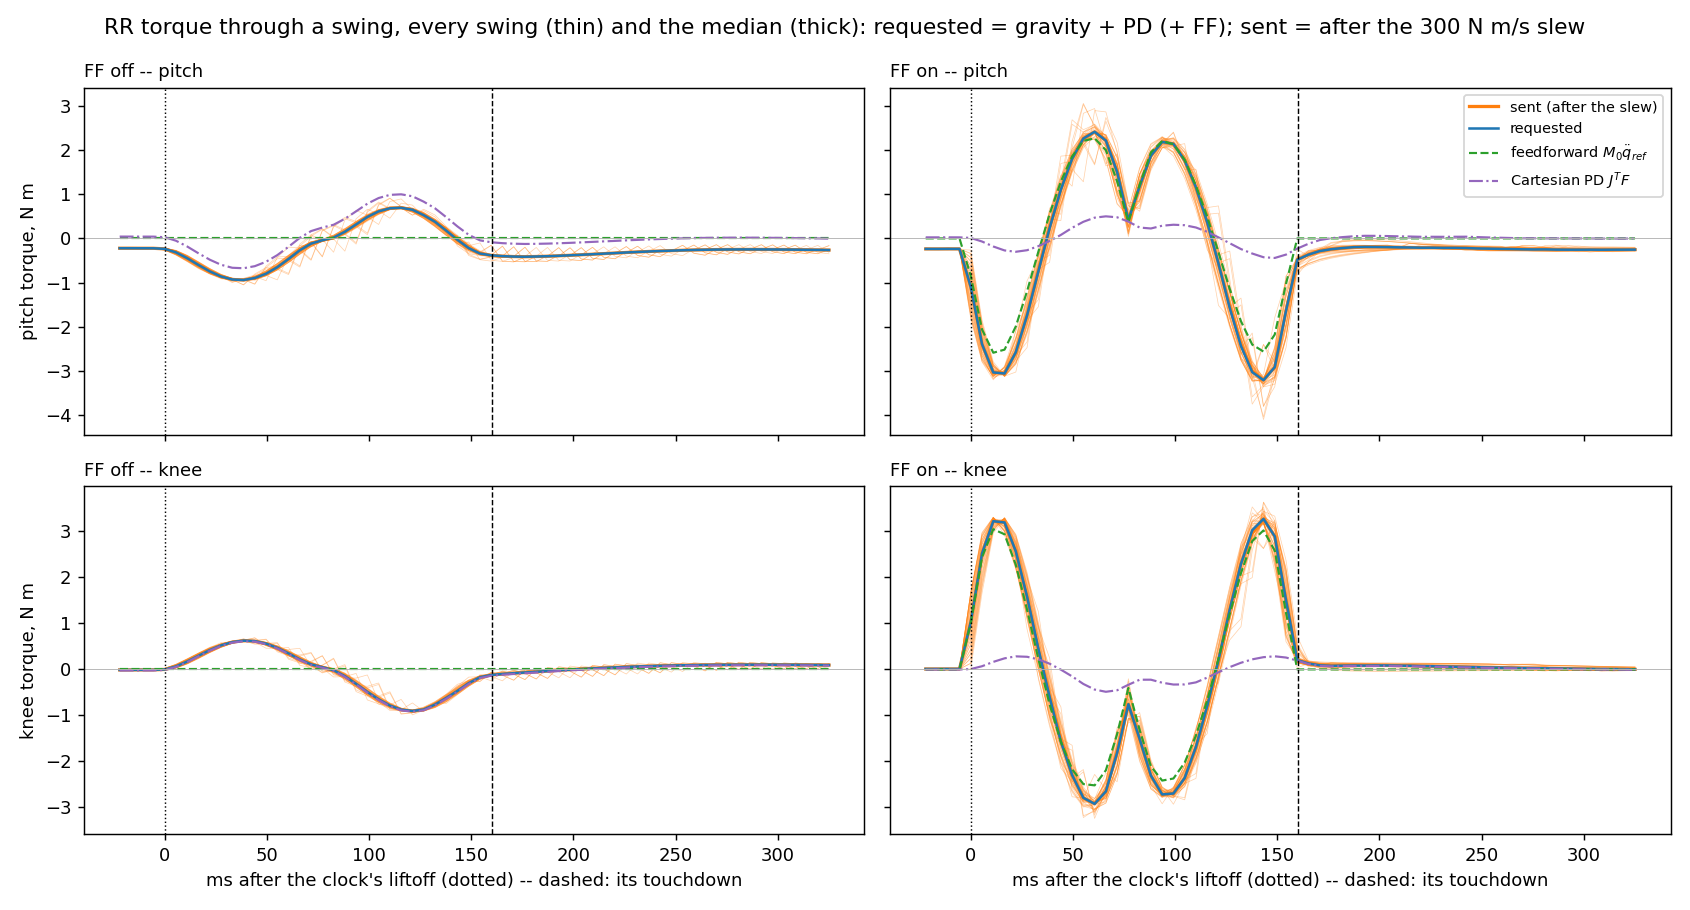
\includegraphics[width=\linewidth]{torque_split.png}
\caption{RR pitch and knee torque through a swing. Thin lines are every swing,
thick lines the median. Off, the request is gravity plus a small PD. On, the
feedforward (green dashed) is almost all of it, and the slew trims the peaks of
what is sent.}
\label{fig:torque}
\vspace{1em}
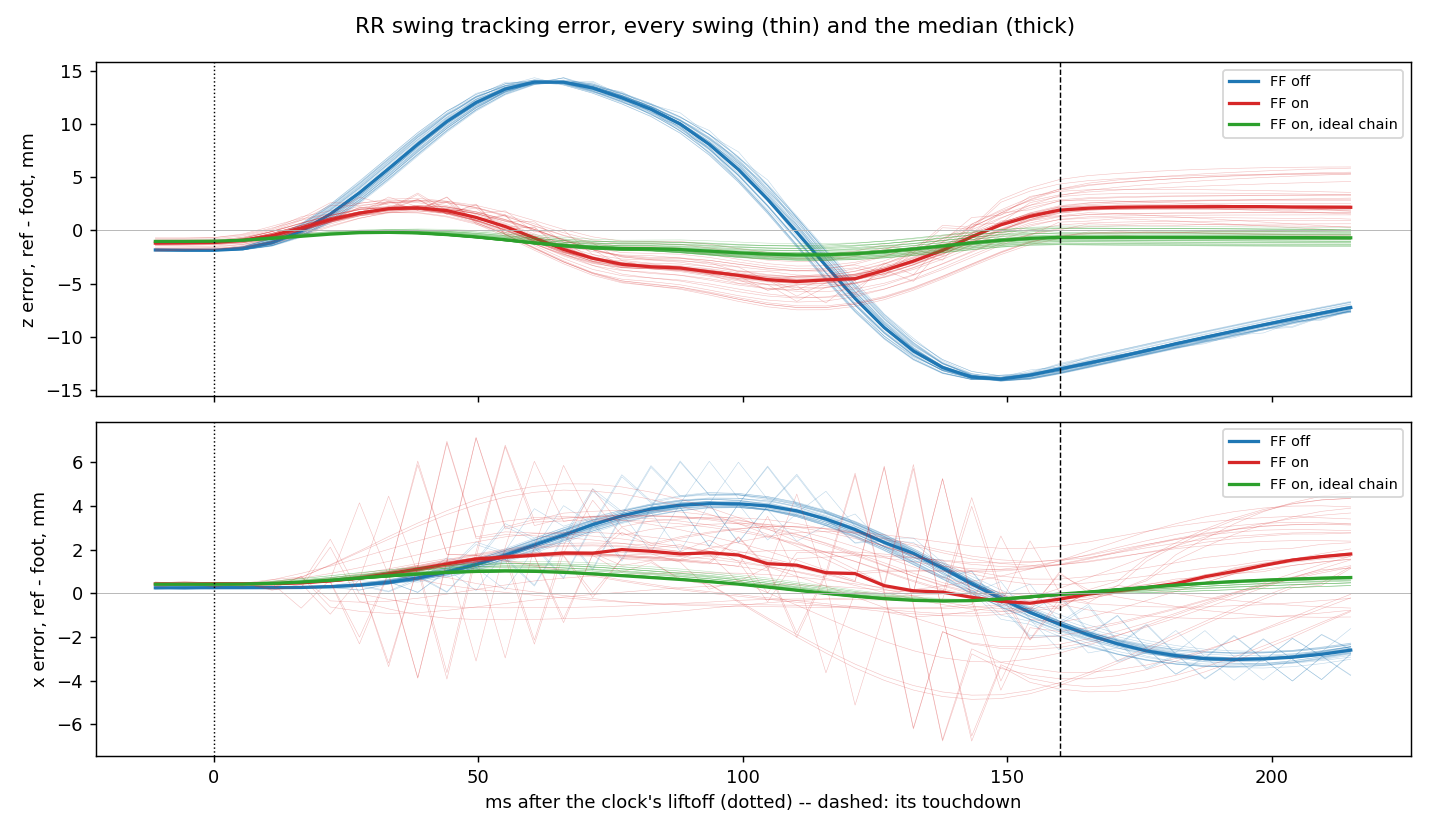
\includegraphics[width=0.92\linewidth]{swing_error.png}
\caption{Tracking error through the swing (the study's figure 18). The $x$
error is the PD's coupling, about 4--5\,mm either way. The sweep-to-sweep
zig-zag is the status request skipping a motor's command.}
\label{fig:err}
\end{figure}

\begin{figure}[h]
\centering
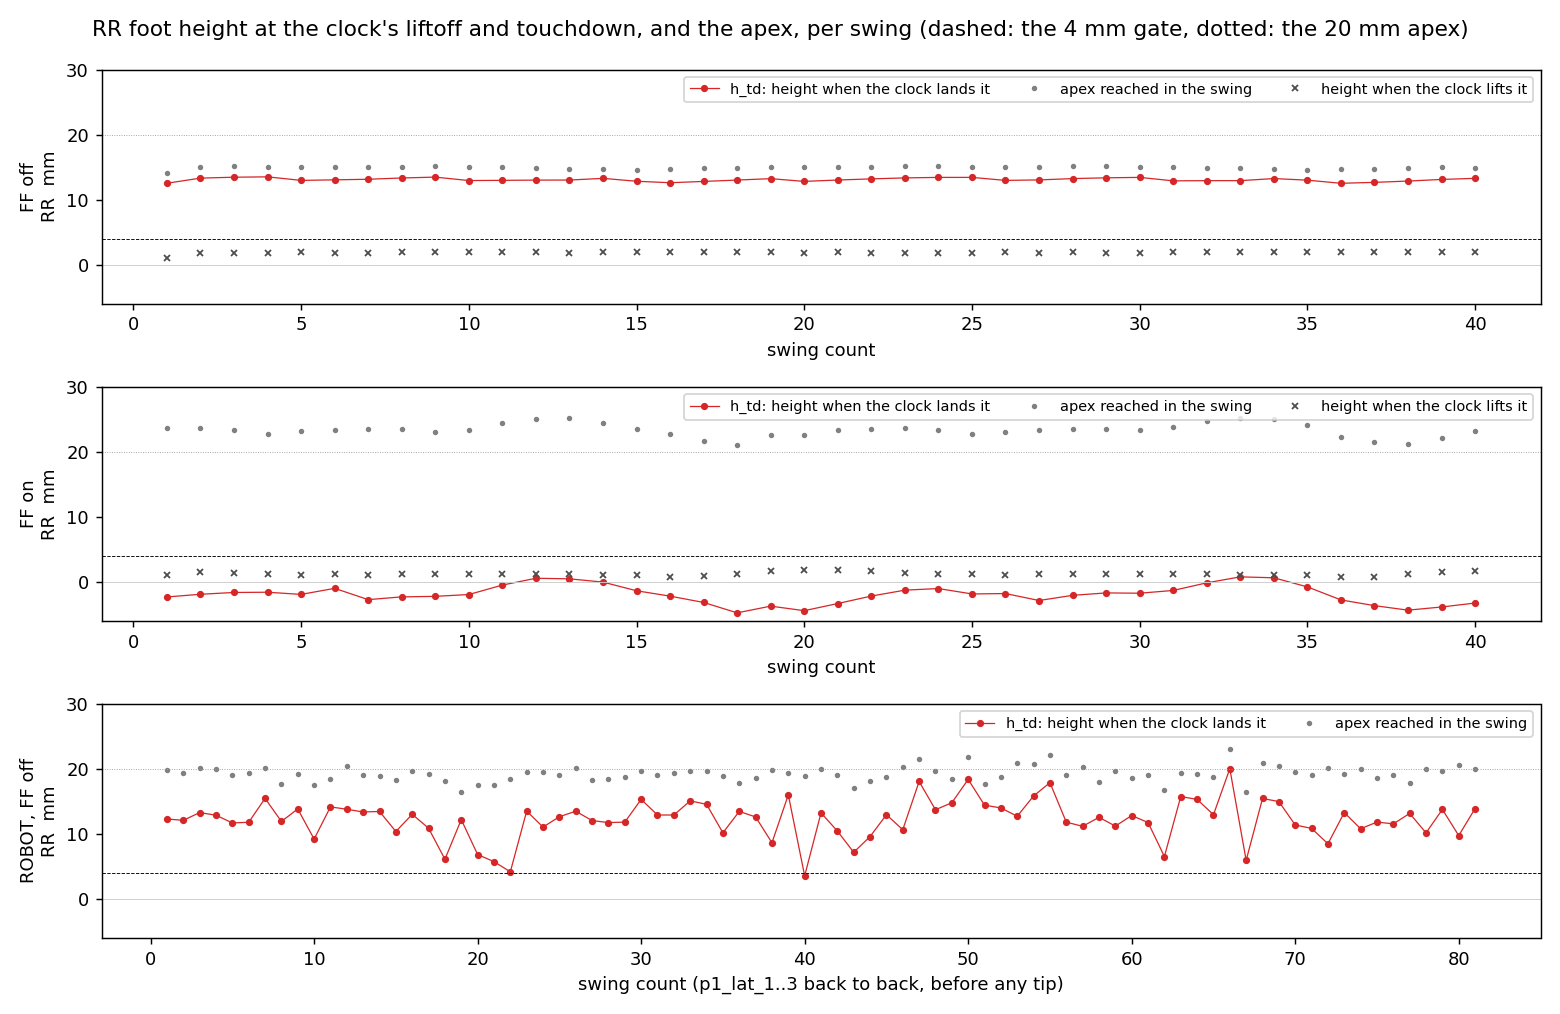
\includegraphics[width=\linewidth]{htd_per_cycle.png}
\caption{Per swing (the study's figure 7): $h_{td}$, the apex, and the height at
liftoff. Off, $h_{td}$ is about 13\,mm on every swing, on the bench as on the
robot. On, it is about $-2$\,mm: the foot is at its site. The bench's off-case
liftoff height of about 2\,mm is the hold ringing in the air at the PD's
1.3\,Hz.}
\label{fig:cycles}
\end{figure}

% ===========================================================================
\section{Against the robot}
\label{sec:robot}

The study has no FF-on log, but it has \RobN{} RR swings with feedforward off,
from the three lateral runs of 2026-10-21 before each tip (\code{p1\_lat\_1..3},
read through the study's own \code{analyse.Run}). The comparison needs one
correction. On the robot, heights are read above the plane of the planted
feet, and the walk's arc starts at the commanded stance height. In the levelled
frame that is \RobZlo\,mm above the floor at liftoff, and the commanded arc
peaks \RobRefPk\,mm above its start. Robot heights are therefore taken from the
arc's start, the same zero the bench uses. On the study's own absolute scale
the apex is \RobApexAbs\,mm and $h_{td}$ is \RobHtdAbs\,mm.

\begin{table}[h]
\centering\small
\begin{tabular}{lrrrr}
\toprule
 & apex, mm & lag, ms & rms, mm & $h_{td}$, mm \\
\midrule
Robot, FF off (81 swings) & 19.3 [17.7, 20.5] & 50 [44, 56] & 11.9 [10.3, 13.9] & 12.7 [8.5, 15.5] \\
Sim, FF off & 15.0 [14.7, 15.1] & 55 [55, 61] & 9.9 [9.7, 10.0] & 13.0 [12.8, 13.4] \\
Sim, FF on & 23.4 [22.0, 24.8] & 33 [28, 33] & 3.4 [2.8, 4.5] & $-$1.9 [$-$3.8, 0.1] \\
\bottomrule
\end{tabular}

\caption{The robot (feedforward off, on the floor, walking) against the hung-up
leg with the feedforward off and on. Medians, with the 10th and 90th
percentiles.}
\label{tab:robot}
\end{table}

The lag and $h_{td}$ agree: on the robot as in the simulation, the foot rises
50--55\,ms after the clock and is about 12--13\,mm up when the clock lands it
(Figure~\ref{fig:phase}, bottom). The robot's apex is 4\,mm higher, \RobApex{}
against \ApexOff\,mm, and its peak comes about 10\,ms earlier. The leg's
inertia is not a candidate here, because its dominant term is the datasheet
rotor, the same on the robot as in the model. The differences the bench leaves
out are these:
\begin{itemize}[leftmargin=1.5em]
\item the robot's foot leaves the floor and the bench's leaves the air, after a
stance in which the planted leg was loaded and its contact ramp unloaded it;
\item the robot's trunk moves under the swing, and the clearance is read in a
levelled frame against the planted feet;
\item the actuator's real torque per commanded torque, friction and damping
are not identified.
\end{itemize}
These logs cannot separate them. The comparison still makes the main point:
with the feedforward off, the robot's foot is as late as the simulated one and
is loaded as high off the floor.

% ===========================================================================
\section{Sensitivity: rotor, $\Mmat_0$ and joint damping}
\label{sec:sens}

\begin{table}[h]
\centering\small
\begin{tabular}{lrrrrrrrrr}
\toprule
 & apex & $s_{apex}$ & lag & rms & $h_{td}$ & $v_{z,td}$ & $|x|$ & $\hat\tau$ & clip \\
 & mm & & ms & mm & mm & m/s & mm & N\,m & N\,m \\
\midrule
FF off & 15.0 & 0.83 & 55 & 9.9 & 13.0 & $-$0.10 & 4.2 & 0.95 & 0.00 \\
FF on & 23.4 & 0.52 & 33 & 3.4 & $-$1.9 & $-$0.11 & 5.0 & 3.31 & 0.21 \\
FF on, $\mathbf{M}_0 = \mathbf{M}_{\mathrm{MuJoCo}}(\mathbf{q}_{hold})$ & 23.2 & 0.52 & 33 & 3.4 & $-$1.7 & $-$0.11 & 5.2 & 3.30 & 0.21 \\
\midrule
FF off, rotor 0.005 & 18.0 & 0.76 & 55 & 9.8 & 11.6 & $-$0.24 & 3.5 & 1.05 & 0.00 \\
FF on, rotor 0.005, $\mathbf{M}_0$ on 0.0085 & 34.0 & 0.45 & 28 & 12.1 & $-$8.8 & $-$0.08 & 17.3 & 4.15 & 0.78 \\
FF on, rotor 0.005, $\mathbf{M}_0$ on 0.005 & 24.5 & 0.48 & 33 & 3.6 & $-$3.4 & $-$0.10 & 5.7 & 2.61 & 0.00 \\
\midrule
FF off, joint damping 0.1 & 10.0 & 0.79 & 66 & 9.8 & 7.6 & $-$0.09 & 5.0 & 0.96 & 0.00 \\
FF on, joint damping 0.1 & 17.3 & 0.45 & 33 & 4.4 & $-$4.8 & $+$0.02 & 5.8 & 3.50 & 0.23 \\
\bottomrule
\end{tabular}

\caption{The same 20\,mm, 160\,ms swing through the hardware chain, with one
thing changed per row.}
\label{tab:sens}
\end{table}

\begin{figure}[h]
\centering
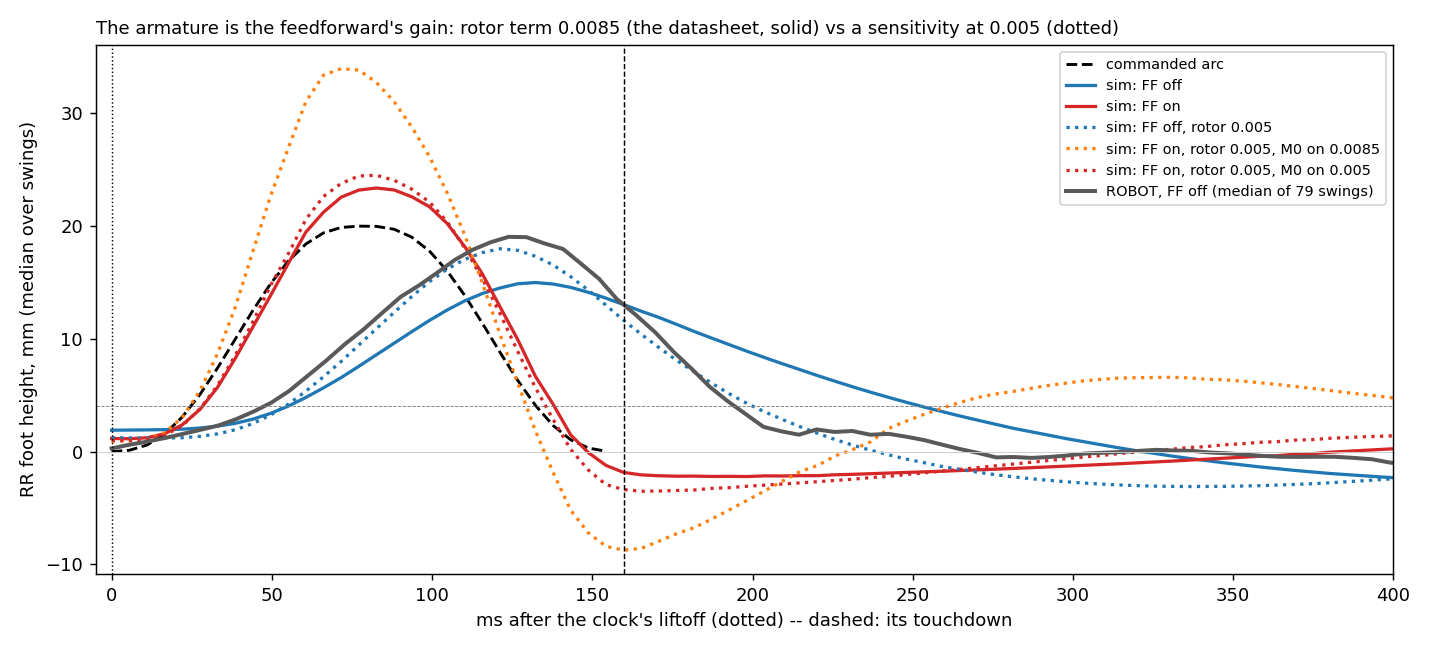
\includegraphics[width=\linewidth]{sensitivity.png}
\caption{Median height through the swing: the datasheet rotor term (solid), the
0.005 sensitivity (dotted), and the robot's FF-off median.}
\label{fig:sens}
\end{figure}

\begin{itemize}[leftmargin=1.5em]
\item \textbf{$\Mmat_0$ from MuJoCo.} Replacing the law's constant with the
weighed leg's $\Mmat(\vq_{hold})$ changes nothing that matters (23.2 against
23.4\,mm). The rotor dominates both.
\item \textbf{An effective inertia below the datasheet's.} The rotor term is
the datasheet value, but the feedforward depends on it so strongly that it is
worth seeing what an error would do. With the plant's rotor term at 0.005 and
$\Mmat_0$ still on 0.0085, the feedforward is about 1.6 times too strong. The
apex is \ApexArmOn\,mm and the rms error \RmsArmOn\,mm; when the clock lands the
foot it is \HtdArmOnAbs\,mm below its site, and it drifts \XArmOn\,mm in $x$.
That resembles the one bench report against the datasheet (2026-09-25: a
15\,mm arc reached 26\,mm and drifted 15--21\,mm in $x$), which is why the
bench check in the next steps is worth one run. Building $\Mmat_0$ on the same
number as the plant restores tracking (\ApexArmMatch\,mm, \RmsArmMatch\,mm rms,
$h_{td}$ \HtdArmMatch\,mm). The feedforward is only as good as the inertia in
it.
\item \textbf{Joint damping}, which neither the model nor the law contains. At
0.1\Nm\,s/rad (the repository's full-robot MJCF value, not a measurement) the
FF-off apex falls to 10\,mm. FF-on still lands on time but reaches only
17\,mm, because the damping eats the feedforward the law does not know to
supply.
\end{itemize}

% ===========================================================================
\section{Conclusions}

\begin{enumerate}[leftmargin=1.5em]
\item With the feedforward off, the 20\,mm, 160\,ms swing is a low-pass
response. The foot reaches 15--19\,mm (simulation and robot), rises 50--55\,ms
late, and is 12--13\,mm in the air when the clock loads it. The robot's logs
show the same timing. This is the late landing the gait study traced its tips
to.
\item With the feedforward on and $\Mmat_0$ matching the leg, the foot follows
the arc. The apex is within 3--5\,mm of $H$ (the overshoot is the chain's), and
the foot is at its site when the clock lands it. The cost is 3.3\Nm{} of peak
torque, well inside the 9\Nm{} clip.
\item The feedforward's gain is the reflected rotor, which is 65--97\,\% of
$\Mmat$. It is the MG5010-i10 datasheet value, shared by DOG5 and DOG6, and the
default $\Mmat_0$ is built on it. Model and plant therefore agree on the term
that matters most. The sensitivity shows how much rides on it: an effective
inertia 40\,\% lower would make the same feedforward overshoot the arc by
70\,\% and bring the foot down hard.
\end{enumerate}

\paragraph{What to do next, in order.}
\begin{enumerate}[leftmargin=1.5em]
\item On the bench, hung up, with these settings and the feedforward on, log
one run (\code{hw.swing\_bench ... --swing-ff --log}). Its apex and $h_{td}$
should be near this note's 23\,mm and $-2$\,mm. \code{--analyse} fits
$\tau - g = I\ddot q + b\dot q + c$ per joint, which checks the effective
inertia against the datasheet and gives the joint damping, which nothing
models yet.
\item Fly the walk with \code{--swing-ff}, keeping the default $\Mmat_0$ unless
the bench fit disagrees with the datasheet. Read the same four numbers in
\code{analyse.py}. $h_{td}$ should fall from about 13\,mm to about 0, with the
apex near 20\,mm.
\item If the 3--5\,mm overshoot matters, it belongs to the chain's 5\,ms delay
and the 300\Nms{} slew, not to the law.
\end{enumerate}

\paragraph{Limits of this note.} The leg swings in air: no floor, no stance load
and no trunk motion. In stance on the bench the foot rings at 1.3\,Hz, which the
floor would stop. The rotor term is the datasheet's. The joint damping and
friction, the actuator's torque accuracy, the driver's current loop and the CAN
timing beyond the measured sweep period are assumed, not identified. The robot
comparison is feedforward-off only, because no FF-on walk log exists.

% ===========================================================================
\appendix
\section{Reproducing this note}

\begin{lstlisting}
set PY=D:\mujoco\.venv\Scripts\python.exe
%PY% doc\swing_height\build_leg.py          # model/leg_RR.xml and its gate
%PY% doc\swing_height\study.py              # 10 runs (~40 s): results.txt,
                                            #   tex/*.tex, fig/*.png
%PY% doc\swing_height\study.py --figures    # tables and figures from data/
latexmk -pdf doc\dog6_swing_height.tex
\end{lstlisting}

\begin{tabbing}
\hspace{4.2cm}\=\kill
\code{model/leg\_RR.xml} \> the plant (generated; \S\ref{sec:model}) \\
\code{build\_leg.py} \> builds it and gates it against \code{hw.kinematics} \\
\code{hwsim\_leg.py} \> \code{SwingBench} on MuJoCo through the emulated chain (\S\ref{sec:hw2sim}) \\
\code{study.py} \> the cases, the metrics, the robot logs, the tables and figures \\
\code{results.txt} \> every number above, with percentiles \\
\code{data/*.npz} \> each run's per-sweep log
\end{tabbing}

The bench flags the simulation corresponds to are
\code{--legs RR --period 0.8 --duty 0.8 --contact-ramp 0.15 --tau-slew 300
--tau-cap 9 --kp-swing 150 150 400 --kd-swing 6 6 40 --swing-height 20}, with or
without \code{--swing-ff}. The bench has no FOLD2 posture, so the simulation
sets it from outside (\S\ref{sec:hw2sim}).

\begin{figure}[h]
\centering
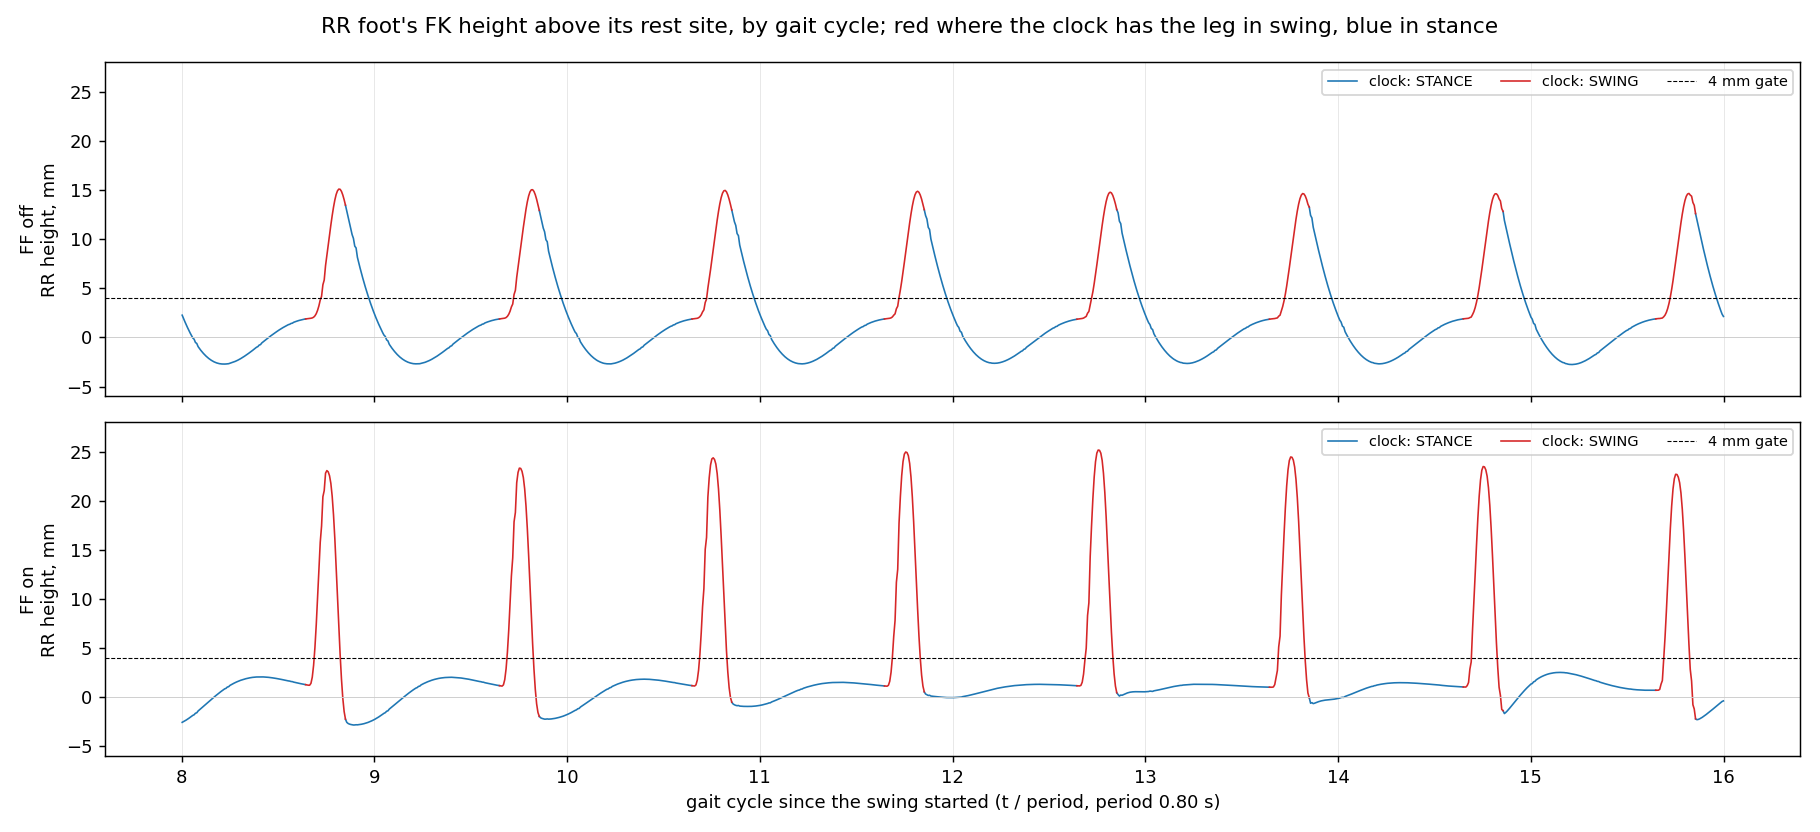
\includegraphics[width=\linewidth]{height_by_gait.png}
\caption{The study's figure 9 for the bench: red where the clock has the leg in
swing, blue in stance.}
\end{figure}

\end{document}
